\documentclass{article}\usepackage[]{graphicx}\usepackage[]{xcolor}
% maxwidth is the original width if it is less than linewidth
% otherwise use linewidth (to make sure the graphics do not exceed the margin)
\makeatletter
\def\maxwidth{ %
  \ifdim\Gin@nat@width>\linewidth
    \linewidth
  \else
    \Gin@nat@width
  \fi
}
\makeatother

\definecolor{fgcolor}{rgb}{0.345, 0.345, 0.345}
\newcommand{\hlnum}[1]{\textcolor[rgb]{0.686,0.059,0.569}{#1}}%
\newcommand{\hlsng}[1]{\textcolor[rgb]{0.192,0.494,0.8}{#1}}%
\newcommand{\hlcom}[1]{\textcolor[rgb]{0.678,0.584,0.686}{\textit{#1}}}%
\newcommand{\hlopt}[1]{\textcolor[rgb]{0,0,0}{#1}}%
\newcommand{\hldef}[1]{\textcolor[rgb]{0.345,0.345,0.345}{#1}}%
\newcommand{\hlkwa}[1]{\textcolor[rgb]{0.161,0.373,0.58}{\textbf{#1}}}%
\newcommand{\hlkwb}[1]{\textcolor[rgb]{0.69,0.353,0.396}{#1}}%
\newcommand{\hlkwc}[1]{\textcolor[rgb]{0.333,0.667,0.333}{#1}}%
\newcommand{\hlkwd}[1]{\textcolor[rgb]{0.737,0.353,0.396}{\textbf{#1}}}%
\let\hlipl\hlkwb

\usepackage{framed}
\makeatletter
\newenvironment{kframe}{%
 \def\at@end@of@kframe{}%
 \ifinner\ifhmode%
  \def\at@end@of@kframe{\end{minipage}}%
  \begin{minipage}{\columnwidth}%
 \fi\fi%
 \def\FrameCommand##1{\hskip\@totalleftmargin \hskip-\fboxsep
 \colorbox{shadecolor}{##1}\hskip-\fboxsep
     % There is no \\@totalrightmargin, so:
     \hskip-\linewidth \hskip-\@totalleftmargin \hskip\columnwidth}%
 \MakeFramed {\advance\hsize-\width
   \@totalleftmargin\z@ \linewidth\hsize
   \@setminipage}}%
 {\par\unskip\endMakeFramed%
 \at@end@of@kframe}
\makeatother

\definecolor{shadecolor}{rgb}{.97, .97, .97}
\definecolor{messagecolor}{rgb}{0, 0, 0}
\definecolor{warningcolor}{rgb}{1, 0, 1}
\definecolor{errorcolor}{rgb}{1, 0, 0}
\newenvironment{knitrout}{}{} % an empty environment to be redefined in TeX

\usepackage{alltt}
\IfFileExists{upquote.sty}{\usepackage{upquote}}{}
\begin{document}


\begin{center}
Name: Mahaprasad Mohanty \\
Registration: 24MDT0061 \\
Course: Statistical Inference \\
Code: PMDS503P
Slot: L33+L34
\end{center}

\section{Question 1}
\begin{knitrout}
\definecolor{shadecolor}{rgb}{0.969, 0.969, 0.969}\color{fgcolor}\begin{kframe}
\begin{alltt}
\hlkwd{library}\hldef{(ggplot2)}
\hldef{data} \hlkwb{<-} \hlkwd{data.frame}\hldef{(}
  \hlkwc{Commodity} \hldef{=} \hlkwd{c}\hldef{(}\hlsng{"Food"}\hldef{,} \hlsng{"Rent"}\hldef{,} \hlsng{"Clothes"}\hldef{,} \hlsng{"Education"}\hldef{,} \hlsng{"Miscellaneous"}\hldef{,} \hlsng{"Savings"}\hldef{),}
  \hlkwc{FamilyA} \hldef{=} \hlkwd{c}\hldef{(}\hlnum{10}\hldef{,} \hlnum{25}\hldef{,} \hlnum{4}\hldef{,} \hlnum{13}\hldef{,} \hlnum{2}\hldef{,} \hlnum{17}\hldef{),}
  \hlkwc{FamilyB} \hldef{=} \hlkwd{c}\hldef{(}\hlnum{8}\hldef{,} \hlnum{36}\hldef{,} \hlnum{7}\hldef{,} \hlnum{16}\hldef{,} \hlnum{4}\hldef{,} \hlnum{33}\hldef{)}
\hldef{)}
\hlkwd{pie}\hldef{(data}\hlopt{$}\hldef{FamilyA,} \hlkwc{labels} \hldef{= data}\hlopt{$}\hldef{Commodity,} \hlkwc{main} \hldef{=} \hlsng{"Expenditure of Family A"}\hldef{)}
\end{alltt}
\end{kframe}
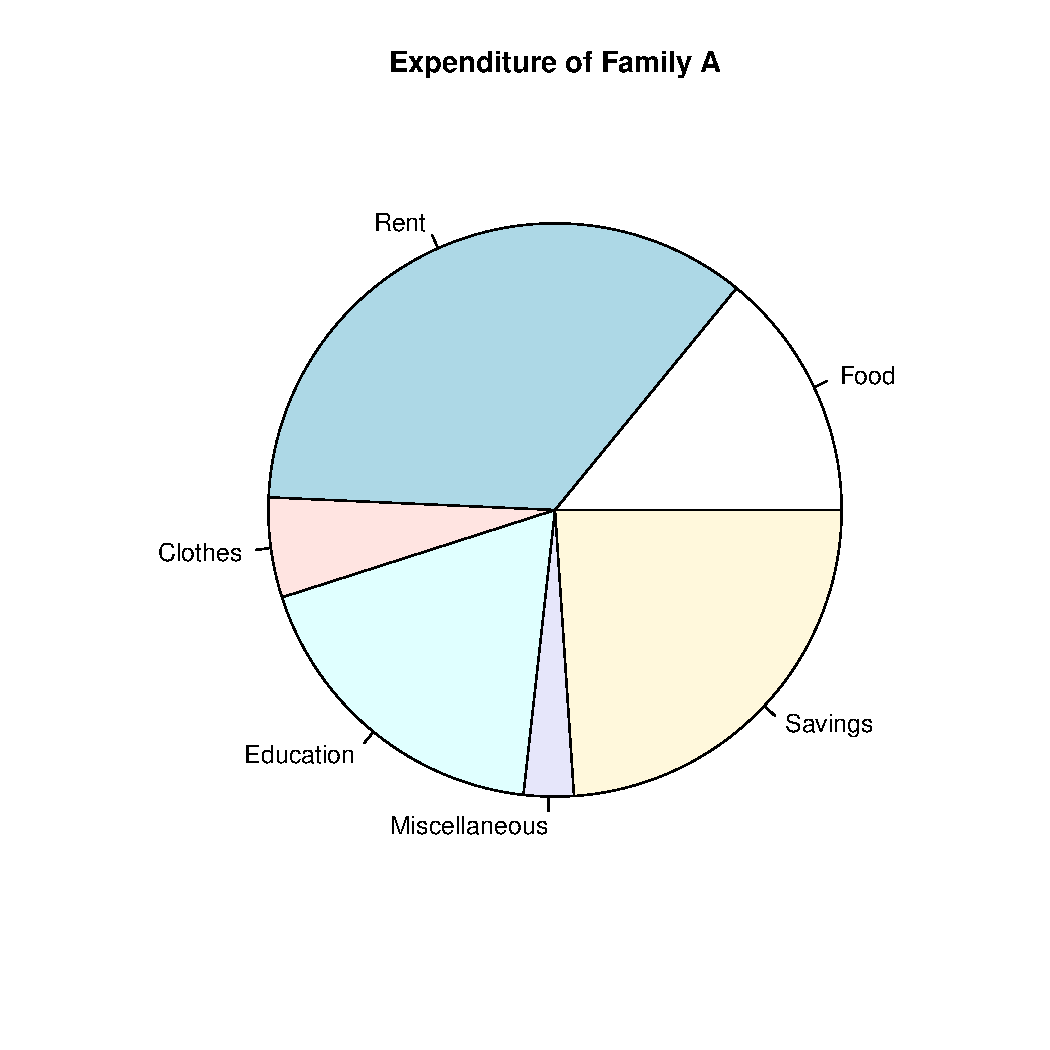
\includegraphics[width=\maxwidth]{figure/unnamed-chunk-1-1} 
\begin{kframe}\begin{alltt}
\hlkwd{pie}\hldef{(data}\hlopt{$}\hldef{FamilyB,} \hlkwc{labels} \hldef{= data}\hlopt{$}\hldef{Commodity,} \hlkwc{main} \hldef{=} \hlsng{"Expenditure of Family B"}\hldef{)}
\end{alltt}
\end{kframe}
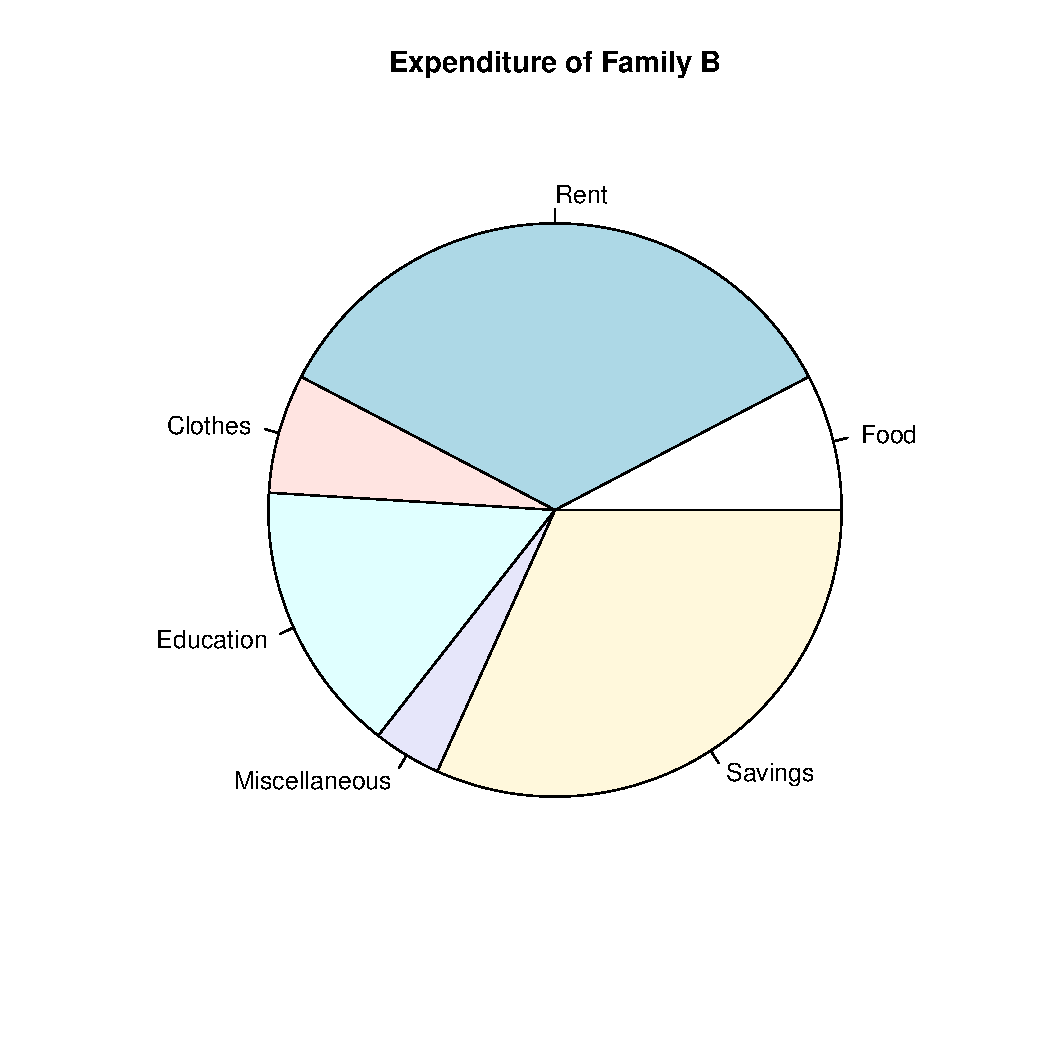
\includegraphics[width=\maxwidth]{figure/unnamed-chunk-1-2} 
\end{knitrout}
\section{Question 2}
\begin{knitrout}
\definecolor{shadecolor}{rgb}{0.969, 0.969, 0.969}\color{fgcolor}\begin{kframe}
\begin{alltt}
\hlkwd{library}\hldef{(MASS)}
\hlkwd{library}\hldef{(ggplot2)}
\hlkwd{data}\hldef{(Boston)}

\hlcom{# (i) Display the number of variables in the dataset}
\hldef{num_variables} \hlkwb{<-} \hlkwd{ncol}\hldef{(Boston)}
\hlkwd{cat}\hldef{(}\hlsng{"Number of variables in the dataset:"}\hldef{, num_variables,} \hlsng{"\textbackslash{}n"}\hldef{)}
\end{alltt}
\begin{verbatim}
## Number of variables in the dataset: 14
\end{verbatim}
\begin{alltt}
\hlcom{# (ii) Draw a box plot for any two variables}
\hlkwd{boxplot}\hldef{(Boston}\hlopt{$}\hldef{crim} \hlopt{~} \hldef{Boston}\hlopt{$}\hldef{chas,}
        \hlkwc{main} \hldef{=} \hlsng{"Box Plot of crim by chas"}\hldef{,}
        \hlkwc{xlab} \hldef{=} \hlsng{"chas"}\hldef{,} \hlkwc{ylab} \hldef{=} \hlsng{"crim"}\hldef{)}
\end{alltt}
\end{kframe}
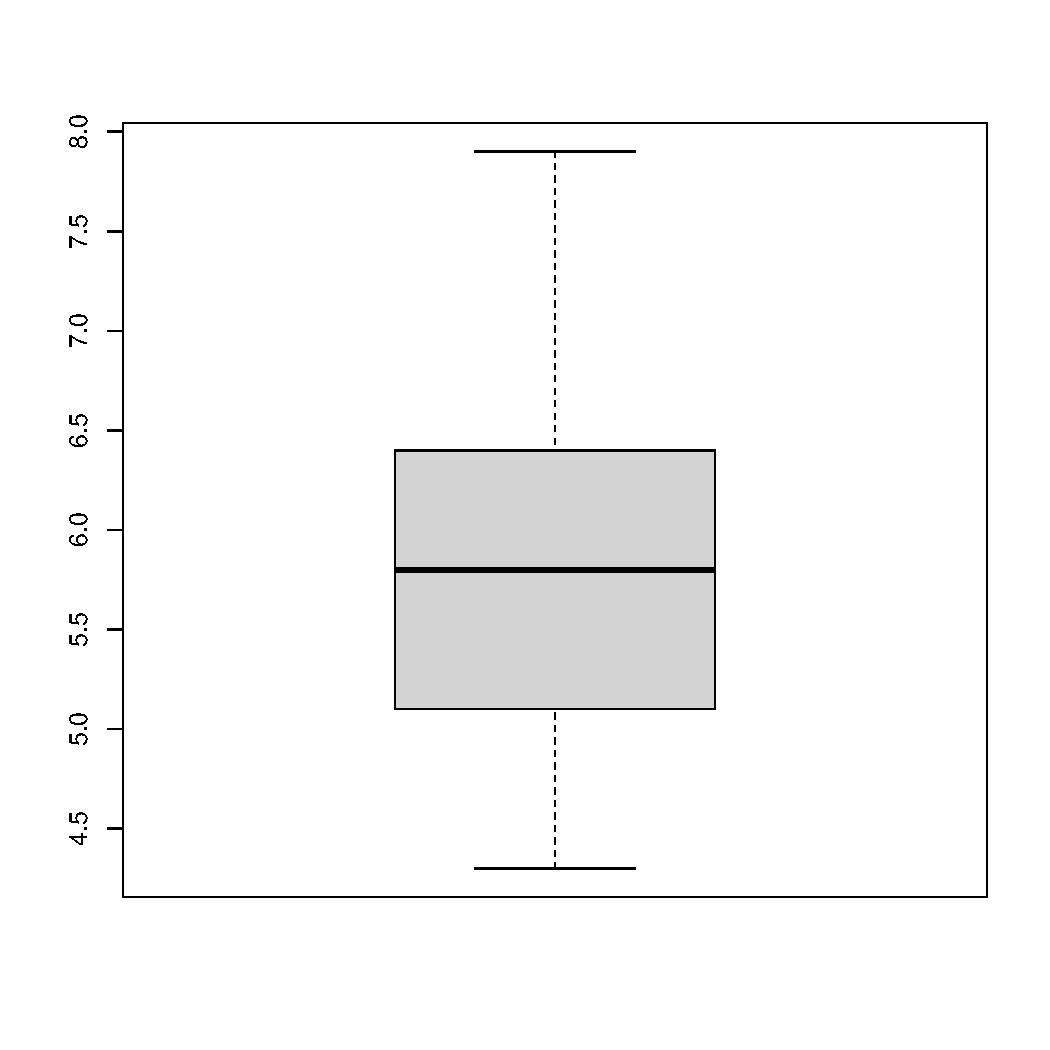
\includegraphics[width=\maxwidth]{figure/unnamed-chunk-2-1} 
\begin{kframe}\begin{alltt}
\hlcom{# (iii) Scatterplot for any two variables}
\hlkwd{plot}\hldef{(Boston}\hlopt{$}\hldef{crim, Boston}\hlopt{$}\hldef{zn,}
     \hlkwc{main} \hldef{=} \hlsng{"Scatterplot of crim vs zn"}\hldef{,}
     \hlkwc{xlab} \hldef{=} \hlsng{"crim"}\hldef{,} \hlkwc{ylab} \hldef{=} \hlsng{"zn"}\hldef{)}
\end{alltt}
\end{kframe}
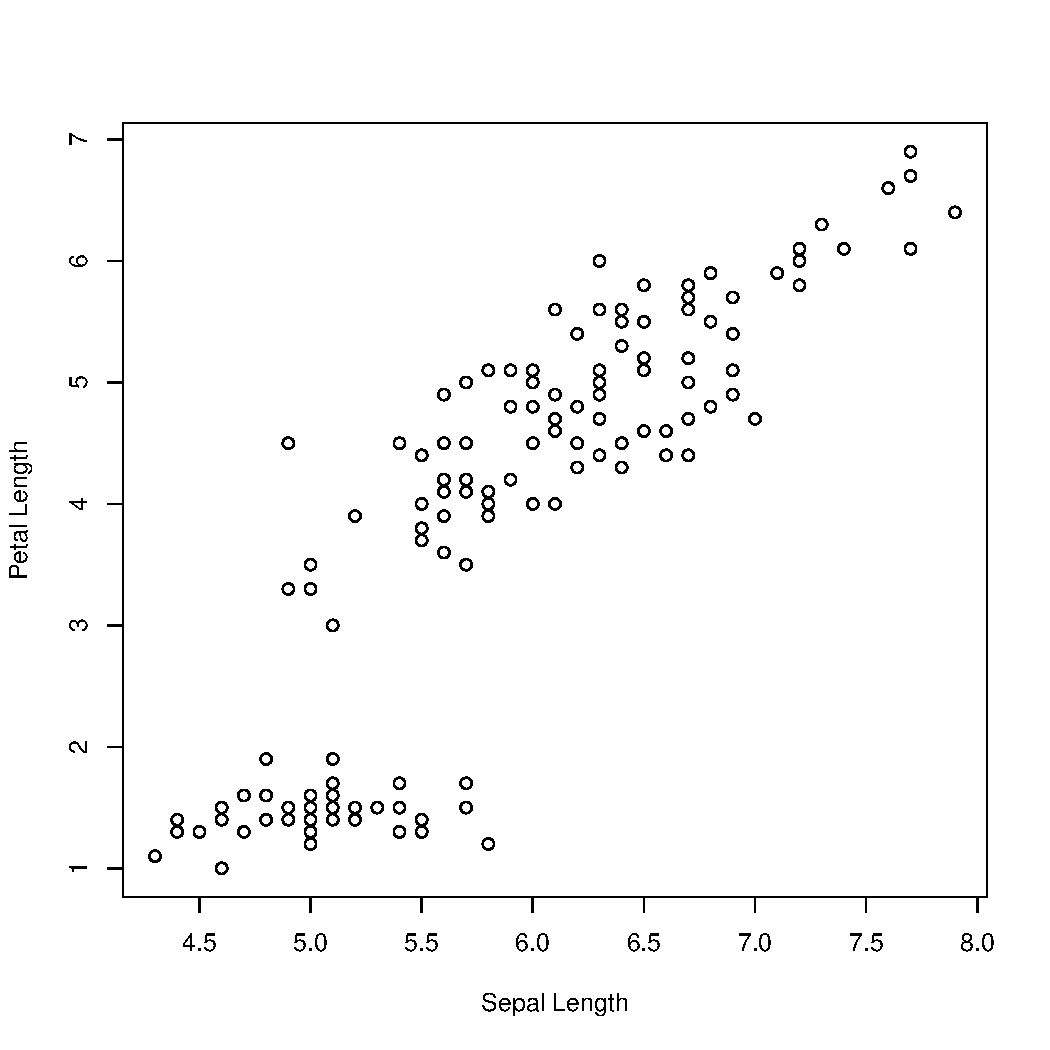
\includegraphics[width=\maxwidth]{figure/unnamed-chunk-2-2} 
\begin{kframe}\begin{alltt}
\hlcom{# (iv) Multiple bar diagram (with different colors)}
\hldef{bar_data} \hlkwb{<-} \hlkwd{data.frame}\hldef{(}
  \hlkwc{variable} \hldef{=} \hlkwd{c}\hldef{(}\hlsng{"crim"}\hldef{,} \hlsng{"zn"}\hldef{),}
  \hlkwc{value} \hldef{=} \hlkwd{c}\hldef{(}\hlkwd{mean}\hldef{(Boston}\hlopt{$}\hldef{crim),} \hlkwd{mean}\hldef{(Boston}\hlopt{$}\hldef{zn))}
\hldef{)}
\hlkwd{ggplot}\hldef{(bar_data,} \hlkwd{aes}\hldef{(}\hlkwc{x} \hldef{= variable,} \hlkwc{y} \hldef{= value,} \hlkwc{fill} \hldef{= variable))} \hlopt{+}
  \hlkwd{geom_bar}\hldef{(}\hlkwc{stat} \hldef{=} \hlsng{"identity"}\hldef{)} \hlopt{+}
  \hlkwd{labs}\hldef{(}\hlkwc{title} \hldef{=} \hlsng{"Multiple Bar Diagram of Mean Values"}\hldef{,}
       \hlkwc{x} \hldef{=} \hlsng{"Variable"}\hldef{,} \hlkwc{y} \hldef{=} \hlsng{"Mean Value"}\hldef{)}
\end{alltt}
\end{kframe}
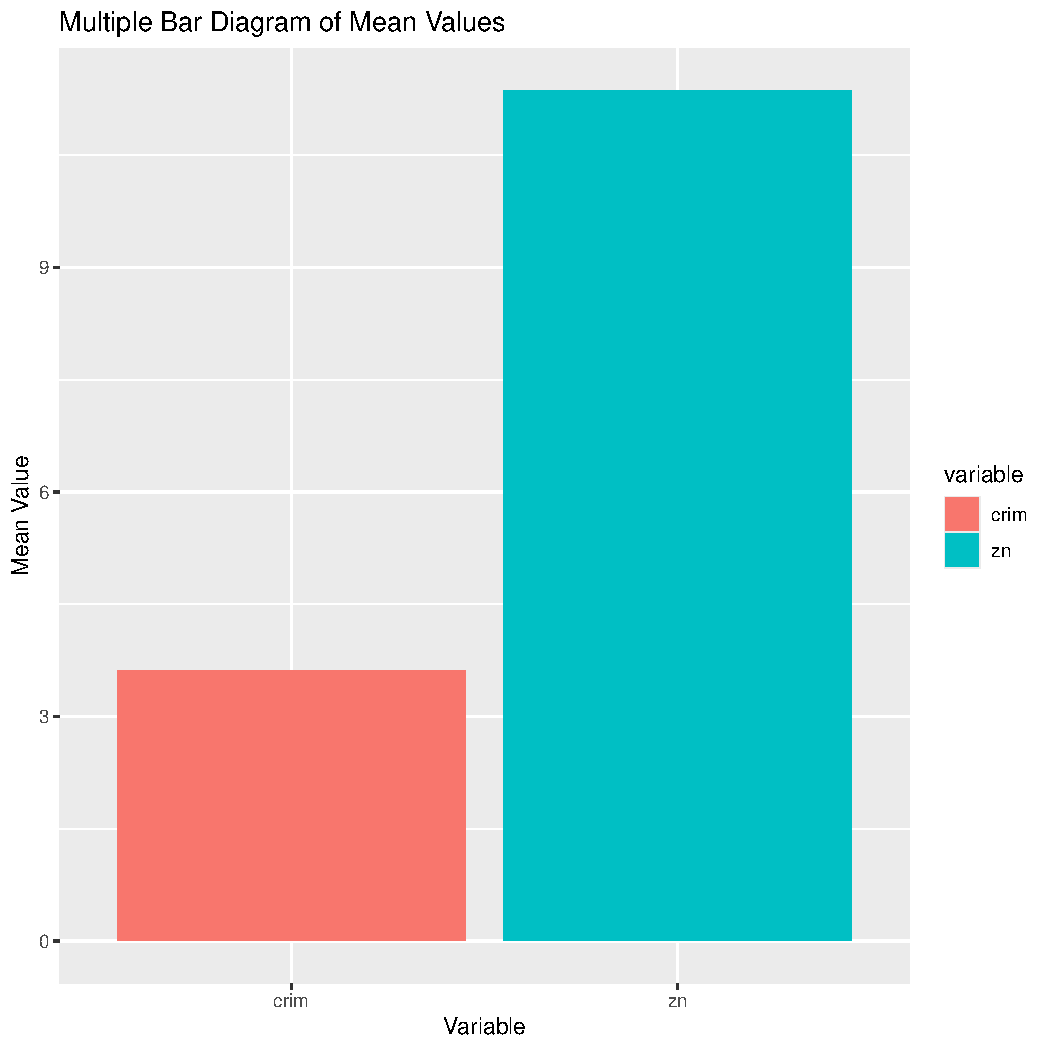
\includegraphics[width=\maxwidth]{figure/unnamed-chunk-2-3} 
\begin{kframe}\begin{alltt}
\hlcom{# (v) Observations}
\hlcom{# - The Boston dataset has 14 variables.\textbackslash{}\textbackslash{}}
\hlcom{# - The boxplot shows that crime rates are very different for 'crim' and 'chas'. There are several outliers in 'chas=0', which suggests a higher crime rate compared to 'chas=1'.\textbackslash{}\textbackslash{}}
\hlcom{# - From the scatter plot, there appears to be no linear relationship between 'crim' and 'zn'.\textbackslash{}\textbackslash{}}
\hlcom{# - From the bar diagram, we can infer that the mean value of 'zn' is much higher compared to the mean value of 'crim'.\textbackslash{}\textbackslash{}}
\end{alltt}
\end{kframe}
\end{knitrout}

\section{Question 3}

\begin{knitrout}
\definecolor{shadecolor}{rgb}{0.969, 0.969, 0.969}\color{fgcolor}\begin{kframe}
\begin{alltt}
\hlkwd{library}\hldef{(dplyr)}
\end{alltt}


{\ttfamily\noindent\itshape\color{messagecolor}{\#\# \\\#\# Attaching package: 'dplyr'}}

{\ttfamily\noindent\itshape\color{messagecolor}{\#\# The following object is masked from 'package:MASS':\\\#\# \\\#\# \ \ \ \ select}}

{\ttfamily\noindent\itshape\color{messagecolor}{\#\# The following objects are masked from 'package:stats':\\\#\# \\\#\# \ \ \ \ filter, lag}}

{\ttfamily\noindent\itshape\color{messagecolor}{\#\# The following objects are masked from 'package:base':\\\#\# \\\#\# \ \ \ \ intersect, setdiff, setequal, union}}\begin{alltt}
\hlkwd{library}\hldef{(xtable)}
\hldef{data} \hlkwb{<-} \hlkwd{read.csv}\hldef{(}\hlsng{'D:\textbackslash{}\textbackslash{}Code-stuff\textbackslash{}\textbackslash{}Stat-Inference\textbackslash{}\textbackslash{}exam-data.csv'}\hldef{)}

\hlcom{# Calculating all summary statistics}

\hlcom{# Mean}
\hldef{mean_CAT1} \hlkwb{<-} \hlkwd{mean}\hldef{(data}\hlopt{$}\hldef{CAT1)}
\hldef{mean_CAT2} \hlkwb{<-} \hlkwd{mean}\hldef{(data}\hlopt{$}\hldef{CAT2)}
\hldef{mean_DA} \hlkwb{<-} \hlkwd{mean}\hldef{(data}\hlopt{$}\hldef{DA)}
\hldef{mean_FAT} \hlkwb{<-} \hlkwd{mean}\hldef{(data}\hlopt{$}\hldef{FAT)}
\hldef{mean_QUIZ1} \hlkwb{<-} \hlkwd{mean}\hldef{(data}\hlopt{$}\hldef{QUIZ1)}
\hldef{mean_QUIZ2} \hlkwb{<-} \hlkwd{mean}\hldef{(data}\hlopt{$}\hldef{QUIZ2)}

\hlcom{# Median}
\hldef{median_CAT1} \hlkwb{<-} \hlkwd{median}\hldef{(data}\hlopt{$}\hldef{CAT1)}
\hldef{median_CAT2} \hlkwb{<-} \hlkwd{median}\hldef{(data}\hlopt{$}\hldef{CAT2)}
\hldef{median_DA} \hlkwb{<-} \hlkwd{median}\hldef{(data}\hlopt{$}\hldef{DA)}
\hldef{median_FAT} \hlkwb{<-} \hlkwd{median}\hldef{(data}\hlopt{$}\hldef{FAT)}
\hldef{median_QUIZ1} \hlkwb{<-} \hlkwd{median}\hldef{(data}\hlopt{$}\hldef{QUIZ1)}
\hldef{median_QUIZ2} \hlkwb{<-} \hlkwd{median}\hldef{(data}\hlopt{$}\hldef{QUIZ2)}

\hlcom{# Minimum and Maximum}
\hldef{min_CAT1} \hlkwb{<-} \hlkwd{min}\hldef{(data}\hlopt{$}\hldef{CAT1)}
\hldef{max_CAT1} \hlkwb{<-} \hlkwd{max}\hldef{(data}\hlopt{$}\hldef{CAT1)}

\hldef{min_CAT2} \hlkwb{<-} \hlkwd{min}\hldef{(data}\hlopt{$}\hldef{CAT2)}
\hldef{max_CAT2} \hlkwb{<-} \hlkwd{max}\hldef{(data}\hlopt{$}\hldef{CAT2)}

\hldef{min_DA} \hlkwb{<-} \hlkwd{min}\hldef{(data}\hlopt{$}\hldef{DA)}
\hldef{max_DA} \hlkwb{<-} \hlkwd{max}\hldef{(data}\hlopt{$}\hldef{DA)}

\hldef{min_FAT} \hlkwb{<-} \hlkwd{min}\hldef{(data}\hlopt{$}\hldef{FAT)}
\hldef{max_FAT} \hlkwb{<-} \hlkwd{max}\hldef{(data}\hlopt{$}\hldef{FAT)}

\hldef{min_QUIZ1} \hlkwb{<-} \hlkwd{min}\hldef{(data}\hlopt{$}\hldef{QUIZ1)}
\hldef{max_QUIZ1} \hlkwb{<-} \hlkwd{max}\hldef{(data}\hlopt{$}\hldef{QUIZ1)}

\hldef{min_QUIZ2} \hlkwb{<-} \hlkwd{min}\hldef{(data}\hlopt{$}\hldef{QUIZ2)}
\hldef{max_QUIZ2} \hlkwb{<-} \hlkwd{max}\hldef{(data}\hlopt{$}\hldef{QUIZ2)}

\hlcom{# Standard deviation}
\hldef{sd_CAT1} \hlkwb{<-} \hlkwd{sd}\hldef{(data}\hlopt{$}\hldef{CAT1)}
\hldef{sd_CAT2} \hlkwb{<-} \hlkwd{sd}\hldef{(data}\hlopt{$}\hldef{CAT2)}
\hldef{sd_DA} \hlkwb{<-} \hlkwd{sd}\hldef{(data}\hlopt{$}\hldef{DA)}
\hldef{sd_FAT} \hlkwb{<-} \hlkwd{sd}\hldef{(data}\hlopt{$}\hldef{FAT)}
\hldef{sd_QUIZ1} \hlkwb{<-} \hlkwd{sd}\hldef{(data}\hlopt{$}\hldef{QUIZ1)}
\hldef{sd_QUIZ2} \hlkwb{<-} \hlkwd{sd}\hldef{(data}\hlopt{$}\hldef{QUIZ2)}

\hlcom{# Printing all}

\hlkwd{cat}\hldef{(}\hlsng{"Summary Statistics:\textbackslash{}n"}\hldef{)}
\end{alltt}
\begin{verbatim}
## Summary Statistics:
\end{verbatim}
\begin{alltt}
\hldef{summary_stats} \hlkwb{<-} \hlkwd{data.frame}\hldef{(}
  \hlkwc{Variable} \hldef{=} \hlkwd{c}\hldef{(}\hlsng{"CAT1"}\hldef{,} \hlsng{"CAT2"}\hldef{,} \hlsng{"DA"}\hldef{,} \hlsng{"FAT"}\hldef{,} \hlsng{"QUIZ1"}\hldef{,} \hlsng{"QUIZ2"}\hldef{),}
  \hlkwc{Mean} \hldef{=} \hlkwd{c}\hldef{(mean_CAT1, mean_CAT2, mean_DA, mean_FAT, mean_QUIZ1, mean_QUIZ2),}
  \hlkwc{Median} \hldef{=} \hlkwd{c}\hldef{(median_CAT1, median_CAT2, median_DA, median_FAT, median_QUIZ1, median_QUIZ2),}
  \hlkwc{Min} \hldef{=} \hlkwd{c}\hldef{(min_CAT1, min_CAT2, min_DA, min_FAT, min_QUIZ1, min_QUIZ2),}
  \hlkwc{Max} \hldef{=} \hlkwd{c}\hldef{(max_CAT1, max_CAT2, max_DA, max_FAT, max_QUIZ1, max_QUIZ2),}
  \hlkwc{SD} \hldef{=} \hlkwd{c}\hldef{(sd_CAT1, sd_CAT2, sd_DA, sd_FAT, sd_QUIZ1, sd_QUIZ2)}
\hldef{)}

\hlcom{# printing the table of summary statistics using xtable library}
\end{alltt}
\end{kframe}
\end{knitrout}

% latex table generated in R 4.4.2 by xtable 1.8-4 package
% Wed Feb 12 21:23:28 2025
\begin{table}[ht]
\centering
\begin{tabular}{lrrrrr}
  \hline
Variable & Mean & Median & Min & Max & SD \\ 
  \hline
CAT1 & 22.35 & 21.00 &   5 &  45 & 9.44 \\ 
  CAT2 & 31.53 & 34.00 &   0 &  49 & 10.67 \\ 
  DA & 10.00 & 10.00 &  10 &  10 & 0.00 \\ 
  FAT & 60.44 & 60.00 &   0 &  94 & 20.90 \\ 
  QUIZ1 & 12.68 & 12.00 &   6 &  20 & 2.96 \\ 
  QUIZ2 & 13.74 & 14.00 &   0 &  20 & 3.38 \\ 
   \hline
\end{tabular}
\caption{Summary Statistics} 
\end{table}







\end{document}


